\chapter{Estado da arte}
\minitoc
% \label{chap:Estadodaarte}
% \vspace{0.5cm}

%%%%%%%%%%%%%%%%%%%%%%%%%%%%%%%%%%%%%%%%%%%%%%%%%%%%%%%%%%%%%%%%%%%%%%%%%%%%%%%%
% Objetivo:                        %
%%%%%%%%%%%%%%%%%%%%%%%%%%%%%%%%%%%%%%%%%%%%%%%%%%%%%%%%%%%%%%%%%%%%%%%%%%%%%%%%

  \lettrine{N}{este} capítulo mostrarase cómo as federacións deportivas están 
xestionando actualmente as súas competicións, cales son as diversas 
alternativas no mercado para isto e tamén se fará unha análise do software 
libre neste campo.

  Búscase mostrar a forte necesidade existente de impulsar unha alternativa 
libre e con boa usabilidade que actualmente está a reclamar o mercado para a 
xestión de actas electrónicas.

  \section{A xestión de competicións e actas deportivas}
  A xestión de competicións e eventos deportivos é unha tarefa que dende fai 
moito tempo se ven realizando de xeito manual e nos últimos anos comezan a 
aparecer no mercado as primeiras aplicacións para facilitar este traballo.

  O proceso comeza cando os xogadores son inscritos a través do seu 
equipo, nunha competición que xestiona unha federación ou asociación 
deportiva. Cando os clubes realizan o pago da inscrición, reciben unha ficha 
identificativa\footnote{É un documento con fotografía e similar ao DNI que 
permite identificar ao integrante do equipo} para cada xogador e persoal do 
mesmo e que deberán levar aos encontros para poder participar.

  Unha vez tódolos equipos están inscritos, a federación procede a crear un 
calendario que contén unha listaxe de enfrontamentos a realizar entre os 
equipos.

  Semanalmente os árbitros da federación son asignados aos partidos que durante 
esa semana se disputa e deben pasar polo local da mesma para recoller un 
modelo en papel da acta dos encontros similar ao que se mostra 
na Figura~\ref{fig:img:acta} e para coñecer os partidos que terán ao 
seu cargo, a data e a localización.

  O árbitro débese desplazar ao campo ou pista onde se disputa o encontro, 
recolle as fichas dos xogadores de ambos equipos e copia dentro da acta aqueles 
que están presentes, descartando os que non asistiron.

    \begin{figure}[h]
          \begin{center}
            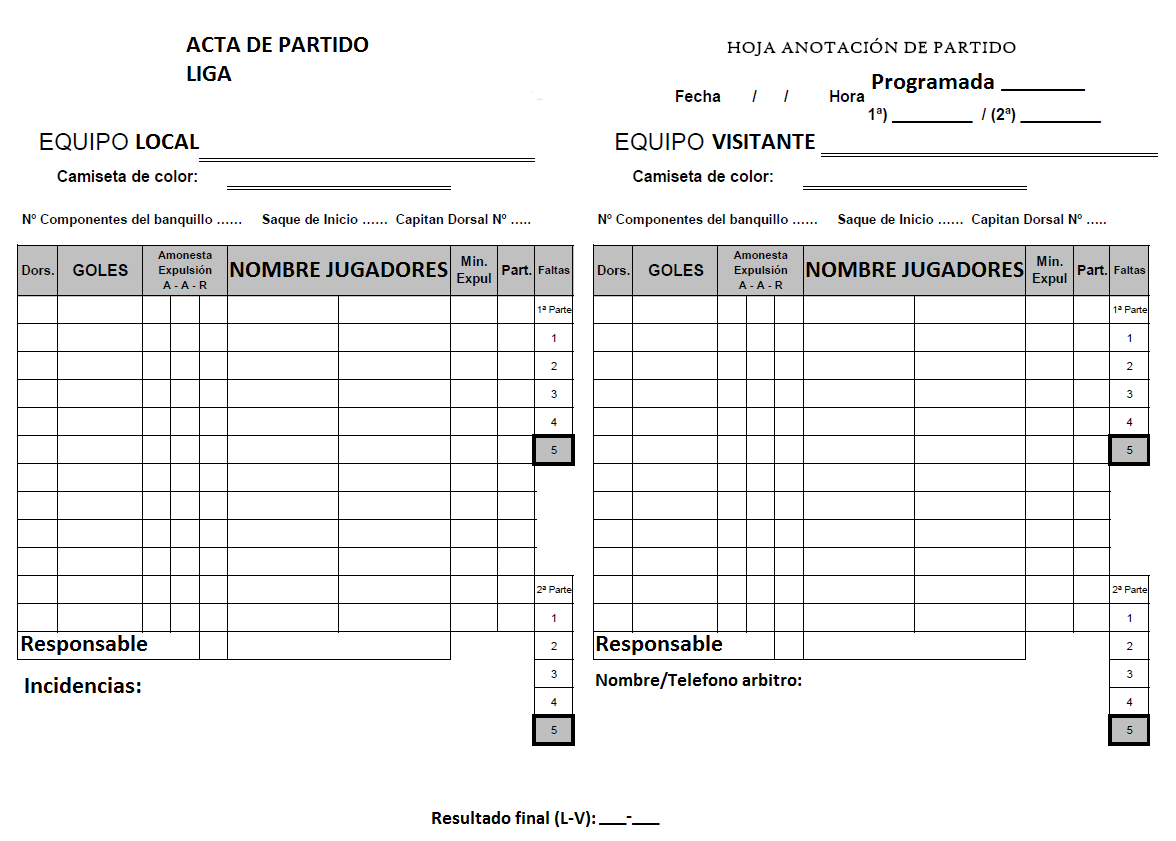
\includegraphics[width=0.8\textwidth]{./img/acta.png}
            \caption{Exemplo de acta deportiva.}
            \label{fig:img:acta}
          \end{center}
    \end{figure}

  Durante o partido o árbitro, ou o segundo árbitro segundo corresponda, 
encárgase de ir cubrindo tódolos eventos que se producen durante o xogo, por 
exemplo goles, faltas, etc.

  Unha vez rematado, os capitáns ou adestradores de ambos equipos deben revisar 
a acta e asinala se están de acordo co que alí se indica, para que 
posteriormente o árbitro traslade unha copia da mesma ao local da federación.

  Alí os empregados da federación rematan o proceso revisando as actas e 
introducindo os datos nunha ferramenta de xestión como as que se comentan no 
seguinte apartado, co fin de actualizar os resultados e a clasificación e para 
finalmente publicalos na páxina web da federación.

  \section{Competidores no mercado}
  Como se comentaba anteriormente, existen diversas ferramentas para xestionar 
competicións, unhas máis avanzadas ca outras pero igualmente funcionais e que 
se van a introducir a continuación, resaltando certas vantaxes e carencias 
das mesmas.

    \subsection{Follas de cálculo}
    A folla de cálculo é o sistema utilizado por excelencia para 
xestionar competicións.

    Un sistema rudimentario pero funcional, algunas federacións combinan en certa medida 
follas de cálculo e bases de datos sinxelas para crear as táboas das 
clasificacións e dos resultados, utilizando funcións que permiten automatizar algunhas 
tarefas como por exemplo o cálculo da clasificación dos equipos en función dos 
seus resultados ao longo da competición.

    \begin{figure}[h!]
	  \begin{center}
	    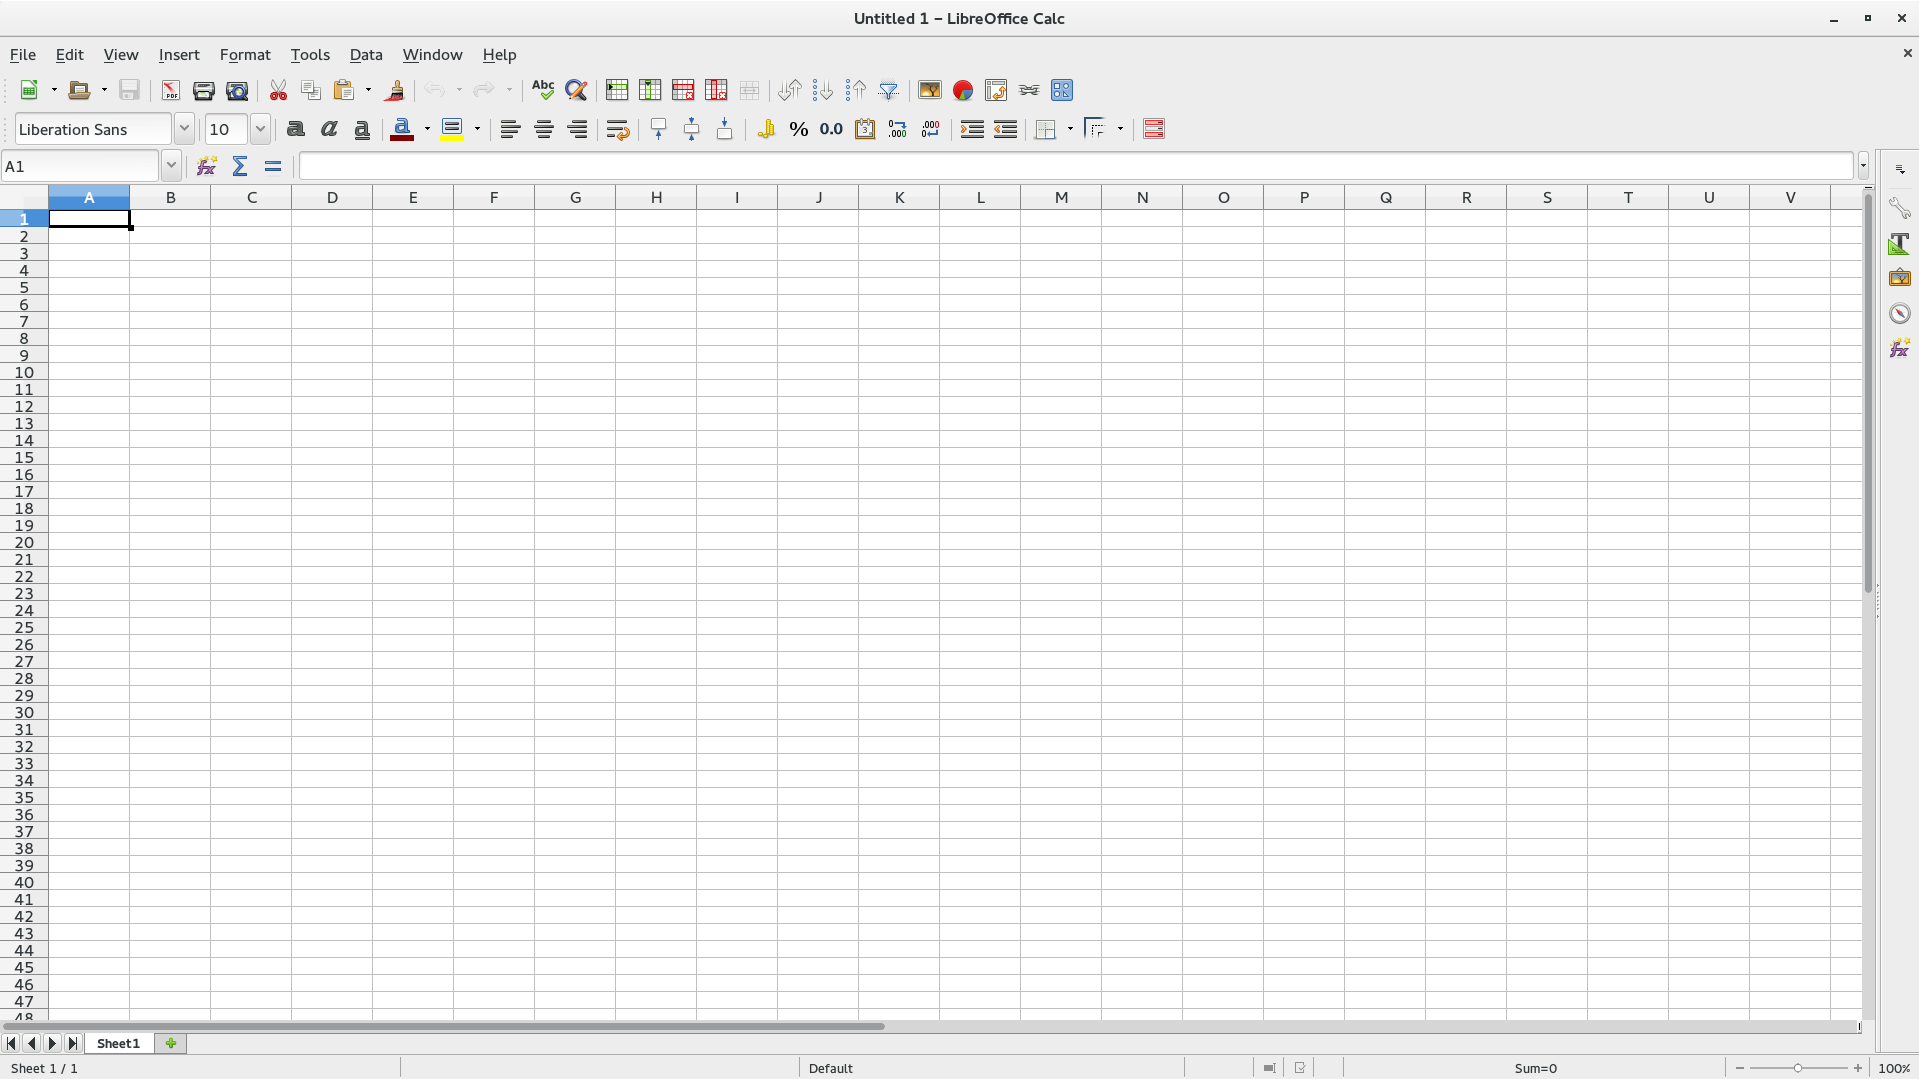
\includegraphics[width=0.8\textwidth]{./img/calculo.png}
	    \caption{Folla de cálculo}
	    \label{fig:img:calculo}
	  \end{center}
    \end{figure}

    O sistema é moi versatil para usuarios experimentados xa que permite adaptar 
as posibles necesidades variables da federación, na forma de calcular 
datos estadísticos, na forma en que se organizan as diferentes competicións, 
etc pero implica un gran traballo manual e pode chegar a ser un suplicio para 
usuarios con poucos coñecementos de ofimática.

  As actas seguen a chegar en papel a federación e os datos deben ser introducidos nas 
diversas follas de cálculo (que en competicións de gran tamaño, vólvense inmanexables), 
revisando as sancións de xeito manual, polo que os erros na interpretación dos datos son 
habituais e por suposto os resultados non son mostrados en tempo real.

    \subsection{Ferramentas tradicionais}

    Tradicionalmente existiron varias ferramentas que comparten características 
de aplicacións web clásicas xa que son solucións especializadas que deben ser 
instaladas invidualmente para cada federación e personalizadas para cada unha a 
través dunha labor de consultoría.

    A continuación imos presentar as dúas alternativas máis extendidas no 
panorama nacional.

      \subsubsection{Novanet}
      Novanet é unha empresa especializada na xestión de competicións de fútbol 
e o seu producto componse únicamente dunha aplicación web dende a que crear as 
clasificacións pero tamén modificar as actas dos partidos ou ver os resultados.

      No caso que nos incumbe, non dispón dunha aplicación que poida ser instalable nun 
teléfono móbil e os árbitros vense na obriga de acceder directamente a páxina web da 
federación para modificar as actas, pero que cando menos adáptase correctamente 
a terminais de menor tamaño como se pode observar na 
Figura~\ref{fig:img:novanet}.

      Ademais, non permite o funcionamento do sistema de forma offline xa que 
non foi pensado inicialmente para o caso, o que obriga a levar a acta en papel 
que se cubre igualmente a pesar de que o árbitro sube posteriormente os datos a 
través da web cando chega a súa casa.

      A interfaz é bastante complexa, o cal é un problema xa que a meirande parte dos 
árbitros son de avanzada idade e polo tanto resúltalles difícil adaptarse 
aínda que está a mellorar pouco a pouco.

      Por último mencionar que únicamente está pensada para ser utilizada en 
fútbol e fútbol sala.
	
      \begin{figure}[h!]
	\begin{center}
	  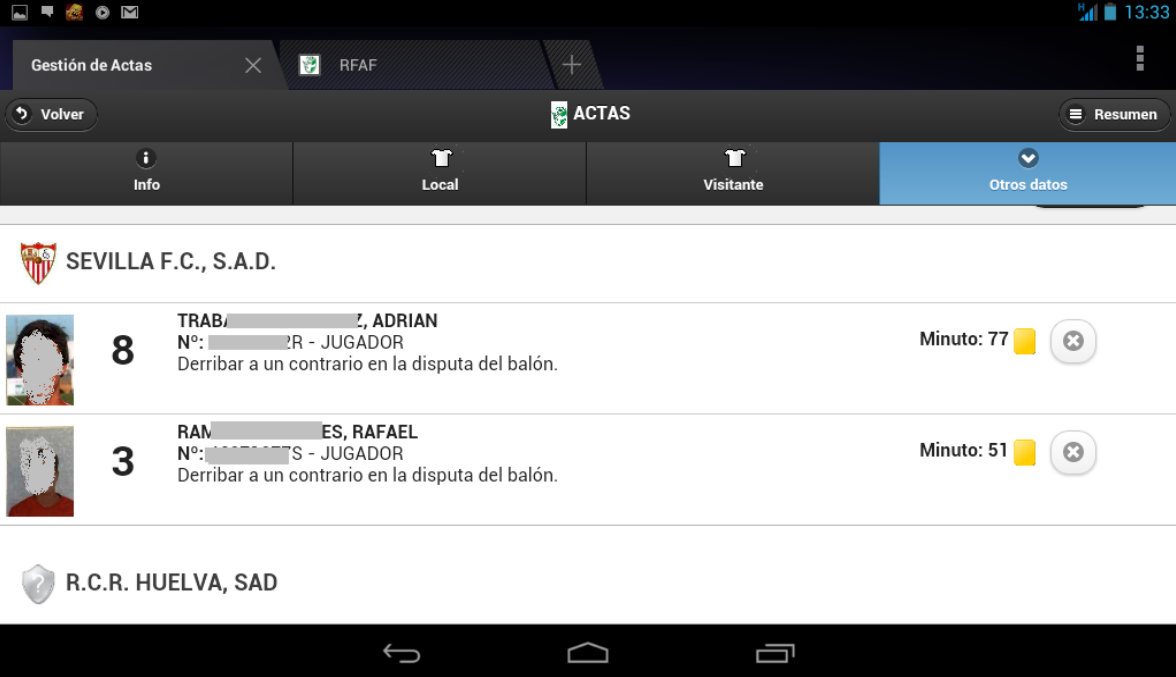
\includegraphics[width=0.8\textwidth]{./img/novanet-app.png}
	  \caption{Aplicación web de Novanet}
	  \label{fig:img:novanet}
	\end{center}
      \end{figure}

    \subsubsection{Federatio}

    O caso de Federatio é moi similiar ao anterior, xa que tampouco dispón 
dunha aplicación específica para a xestión de actas electrónicas de forma 
sinxela e polo tanto, os árbitros deben acceder a través da páxina web ao chegar 
a casa para pasar os datos da acta física á versión electrónica.

    A interfaz dista de ser atractiva xa que apenas se renovou dende que comezou a 
funcionar, entorno ao ano 2005, e non se atopa adaptada para terminais móbiles, 
o que dificulta enormemente a labor dos árbitros.

    A pesar de isto, é unha solución amplamente utilizada en deportes como o 
voleibol e o balonman como se pode observar na Figura~\ref{fig:img:federatio} 
na que podemos observar a páxina web da Federación Galega de Voleibol que 
dispón do sistema Federatio integrado.

      \begin{figure}[h!]
	\begin{center}
	  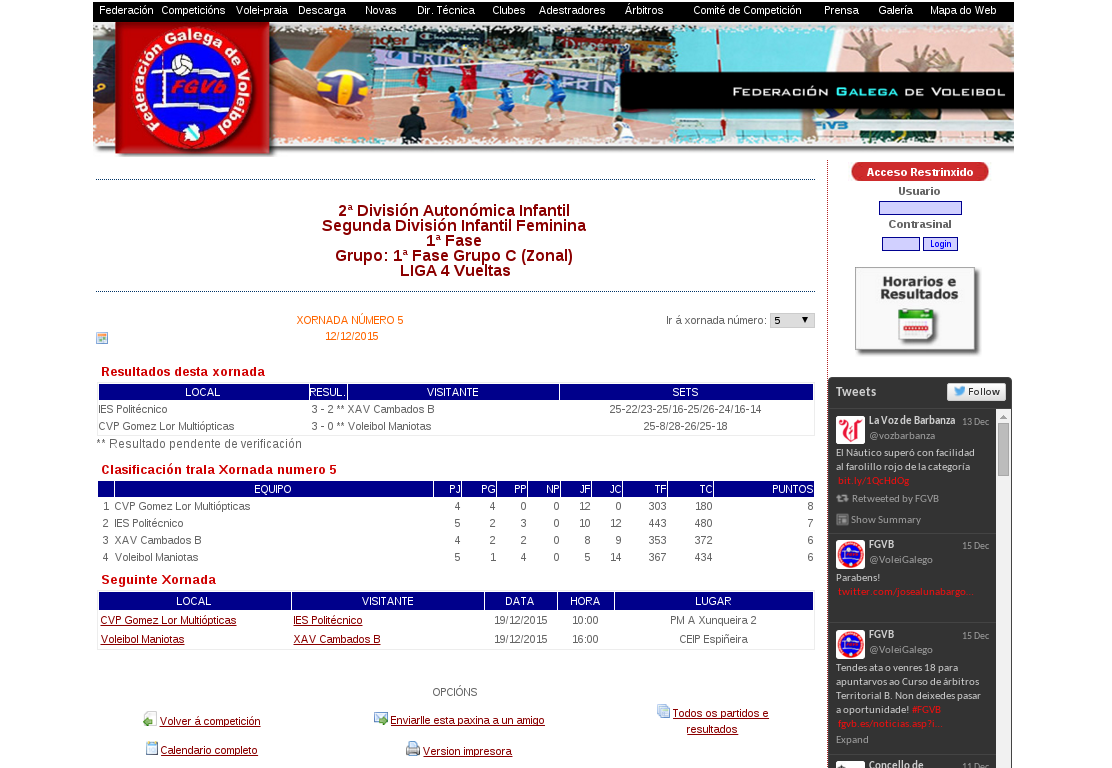
\includegraphics[width=0.8\textwidth]{./img/federatio-app.png}
	  \caption{Web da FGVB co sistema Federatio}
	  \label{fig:img:federatio}
	\end{center}
      \end{figure}

\clearpage


  \subsection{Ferramentas na nube}

  Nos últimos anos xurdiron unha serie de tecnoloxías que democratizaron o 
acceso a nube e por iso xurdiron varias productos específicos e centrados en 
xestionar dende unha única plataforma, múltiples federacións e asociacións 
deportivas.

    \subsubsection{miLeyenda}

    miLeyenda é unha de estas plataformas para a xestión de competicións na 
nube que permite aos administradores de federacións dispor tamén de unha 
aplicación móbil nativa para IOS e outra para Android que se pode ver na 
Figura~\ref{fig:img:mileyenda}.

    Dende esta aplicación poden xestionar gran parte dos parámetros das súas competicións 
entre os que se atopan as clasificacións, as altas de xogadores e por 
suposto, as actas dos encontros.

    Así mesmo tamén dispoñen dunha aplicación para que os xogadores e clubes poidan ver 
os resultados e as clasificacións polo que o custe de mantemento ditas 
aplicacións elévase enormemente ao ter que soportar ata 4 apps móbiles 
diferentes.

    Esta é unha das grandes vantaxes de utilizar as tecnoloxías web que emprega VACmatch 
Mobile, permitíndo utilizar unha soa aplicación para calquera sistema 
operativo e que incluso pode funcionar en un simple navegador web.

    A usabilidade das aplicacións é tamén salientable e permite a xestión de 
diversos deportes pero a cambio non permite de momento cubrir as actas de forma 
offline, un problema habitual ante a falta de cobertura nos diversos pavillóns e 
campos deportivos.

      \begin{figure}[h!]
	\begin{center}
	  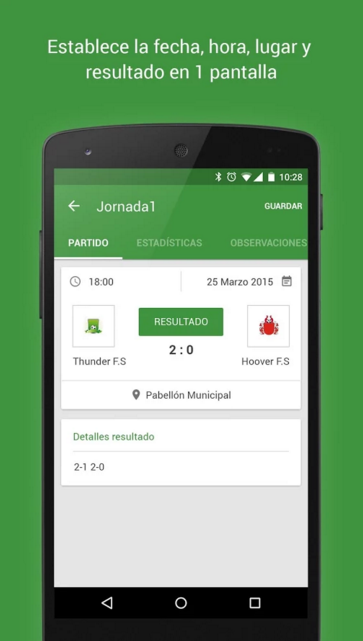
\includegraphics[width=0.3\textwidth]{./img/mileyenda-app.png}
	  \caption{APP móbil de MiLeyenda}
	  \label{fig:img:mileyenda}
	\end{center}
      \end{figure}

    \subsubsection{Esportics}

    Esportics é outra solución tamén española e que se centra na xestión de 
competicións deportivas de tenis, paddel e deportes electrónicos e que lles 
permite aos xestores crear o seu propio espacio dentro do portal como o exemplo 
que temos na Figura~\ref{fig:img:esportics}.

A pesar de que a aplicación funciona para múltiples deportes, a súa adaptación 
é bastante forzada en certos menús e á hora de estruturar as competicións.

    Únicamente dispón dunha páxina web adaptable a móbiles, aínda que a 
adaptación é  tamén mellorable, e non dispón dunha aplicación específica para 
que os árbitros poidan cubrir as actas dende o seu teléfono.

    A usabilidade é aceptable, engadindo unha complexidade 
que non é precisa en certos menús e que provoca que os árbitros de avanzada 
idade, lles resulte tamén pouco intuitivo.

    \begin{figure}[h!]
      \begin{center}
	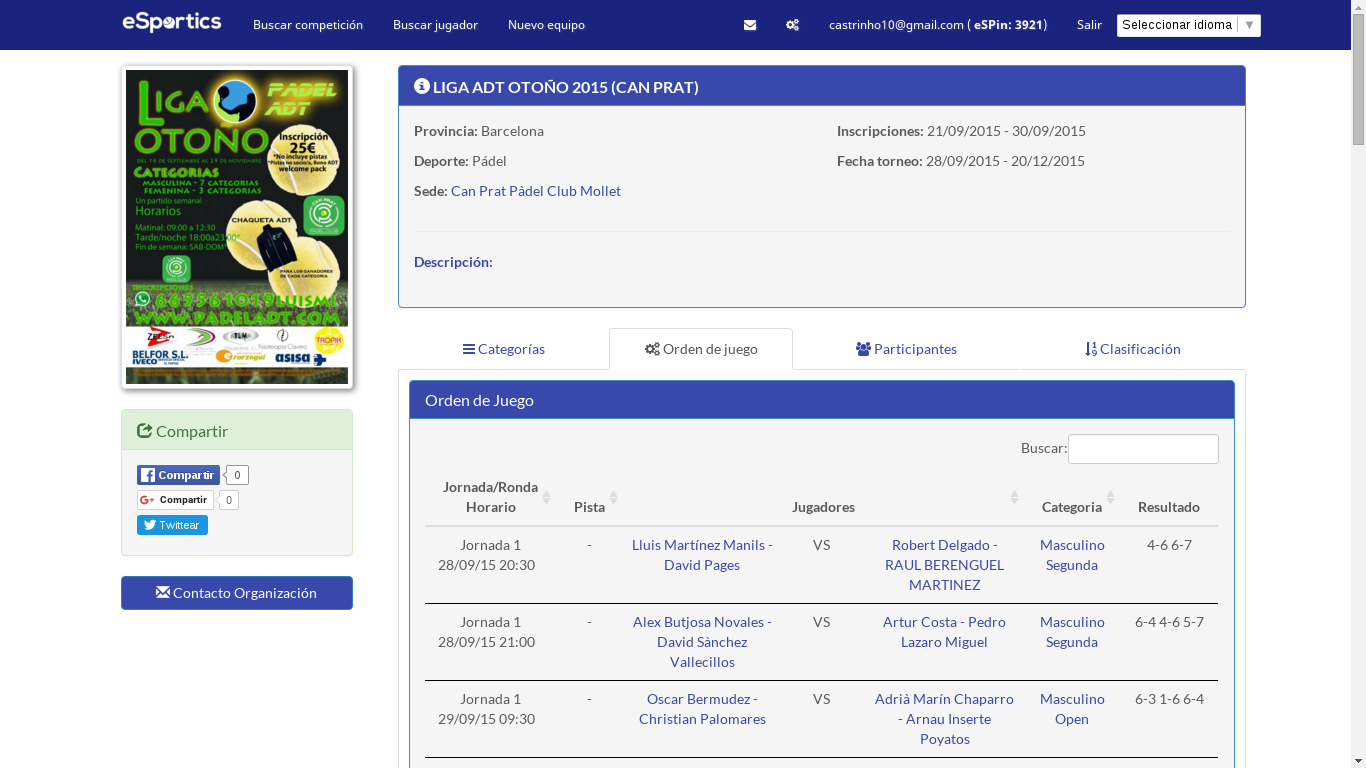
\includegraphics[width=\textwidth]{./img/esportics-app.png}
	\caption{Torneo de tenis na web de Esportics}
	\label{fig:img:esportics}
      \end{center}
    \end{figure}

    \subsubsection{Sportngin}

    Sportngin é unha solución integral para a xestión deportiva, probablemente 
un dos proxectos de referencia xa que dispón de aplicacións web e móbil para a 
xestión e a visualización de competicións.

    De feito, Sportngin permite a personalización da aplicación móbil para 
cada federación, cos seus logotipos, colores corporativos e incluso certos 
menús personalizables, dando a posibilidade de cubrir as actas de forma 
offline, todo con unha interfaz moi amigable como a que podemos ver na 
Figura~\ref{fig:img:sportngin}.

    A parte das funcións habituais para xestionar as competicións e a creación 
de actas, con unha usabilidade moi coidada, aporta como valor engadido a 
visualización e xestión de noticias, fotos ou estadísticas da competición.

    Por último tamén permite aos entrenadores planificar adestramentos e incluso 
comunicarse cos seus xogadores a través da mensaxería interna.

    É sen dúbida o proxecto máis completo e a referencia a seguir a pesar de 
non ser software libre.
 
    \begin{figure}[h!]
      \begin{center}
	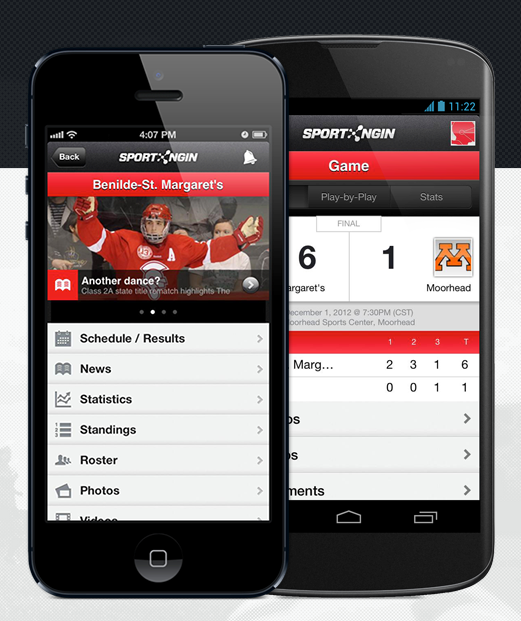
\includegraphics[width=0.5\textwidth]{./img/sportngin-app.png}
	\caption{APP móvil de Sportngin}
	\label{fig:img:sportngin}
      \end{center}
    \end{figure}

    \todo{Engadir taboa comparativa}

    \subsection{Outras plataformas}
    Existen moitas ferramentas para a xestión de competicións e resultados pero apenas 
ningunha facilita aos árbitros unha plataforma sinxela e con unha 
usabilidade coidada.

    Tamén existen pequenos plugins coa idea de extender outras plataformas 
xenéricas para adaptalas a xestión de competicións como o \emph{Joomla! CMS 
sport extension}\footnote{Plugin para o sistema de xestión de contidos Joomla.} 
pero a función final é moi limitada.

    Por último temos outras propostas como \emph{Siguetuliga}\footnote{Rede 
social para o deporte aficionado.} que permite que as persoas que se atopan 
vendo o partido, poidan subir os resultados pero simplemente é un complemento, 
non facilita nin elimina o traballo dos xestores de competicións.

  \section{Aplicacións libres no mercado}

    O software libre é un sector en crecemento na actualidade, os proxectos 
colaborativos que forman o mundo \emph{Open Source} estanse a impor en múltiples 
mercados fronte ás correspondentes alternativas privativas que adoitan a ser 
tremendamente custosas e que atan ao usuario a tecnoloxías pechadas, 
impedíndolle ser o dono real do seu software, sen poder adaptalo ou engadirlle 
novas funcionalidades, nin tan sequera ver cómo se atopa feito e poder 
certificar así a seguridade da súa información.

    Mesmo as grandes compañías TIC están a apostar por liberar parcial ou totalmente as 
súas tecnoloxías e productos, favorecendo un desenvolvemento colaborativo fronte a idea 
atrasada do individualismo do modelo productivo tradicional.

    Concretamente no mundo do deporte é tremendamente complicado atopar algún 
exemplo de aplicación baseada en software libre e as poucas existentes como 
\emph{zuluru} ou \emph{phpmysport} non destacan pola súa usabilidade nin polas 
súas funcionalidades, moi por detrás de outras solucións comerciais como as 
comentadas anteriormente e por suposto sen ningún tipo de aplicación móbil 
para facilitar a xestión das actas polo que é importante propor unha 
alternativa como VACmatch Mobile ás aplicacións privativas.

  \section{Solución aberta e adaptable}
  Os xestores de competicións habitualmente realizan unha considerable inversión 
económica para que unha empresa de consultoría lles cree unha aplicación web ou de 
escritorio a medida para a súa xestión. Algunhas mesmo dispoñen de aplicacións móbiles 
para os árbitros pero que son específicas para dito sistema de xestión polo que a 
reutilización de aplicacións non é posible.

  Ademáis, estos sistemas son propietarios e o código non se atopa accesible 
polo que é imposible tratar de adaptar ditas aplicacións para outros 
sistemas de xestión ou de engadirlles funcionalidades sen depender da empresa 
que comercializa o software.

  É por isto polo que se chegou a conclusión de que é preciso crear unha 
plataforma aberta como é VACmatch Mobile que porporciona unha aplicación 
software libre adaptable a diversos deportes e integra unha API de comunicacións 
aberta para a xestión de actas electrónicas e que permite a súa integración 
noutros sistemas de xestión entre os cales se atopa o sistema de VACmatch Web, 
unha implementación libre para a xestión de competicións.


%%% Local Variables:
%%% mode: latex
%%% TeX-master: "../root"
%%% End:
